\documentclass[t]{beamer}
\usepackage{CJKutf8}
\usepackage{amsfonts}
    \usepackage{amsmath}
    \usepackage{amssymb}
    \usepackage{amsthm}
    \usepackage{enumerate}
    \usepackage{graphicx}
    \usepackage{layout}
    \usepackage{mathrsfs}
    \usepackage{fancyhdr}
    \usepackage{subfigure}
    \usepackage{tcolorbox}
    \usepackage{tikz-cd}
    \usepackage{color}
    \usepackage{pifont}
    \usepackage{verbatim}
    \usepackage{mathtools}
    \usepackage{float}
    \usepackage{bm}
    \usetheme{AnnArbor}
% \usetheme{Antibes}
\usecolortheme{beaver}
\usepackage{listings}


\usepackage{subfigure}

% 添加网址的命令
\usepackage{hyperref}
% 这是一个带链接文本的示例:\href{https://www.example.com}{点击这里访问网站}
% 普通的示例:\url{https://www.example.com}
% 表格
\usepackage{booktabs}
\usepackage{multirow}

% \setbeamertemplate{navigation symbols}{}

\usepackage{textpos}

\newcommand{\dif}{\mathrm{d}}
\newtheorem{thm}{{定理}}

% some common command
\newcommand{\mm}[1]{$ #1$\newline}
% \newcommand{\tuichu}{\Rightarrow}
% \newcommand{\li}[1]{\newline#1}



\newcommand{\analysis}[2]{\forall \mathcal{E}{#1},\exists \delta {#2},s.t.}
\newcommand{\denyanalysis}[2]{\exists \mathcal{E}{#1},\forall \delta {#2},s.t.}
\newcommand{\yield}{\Rightarrow }
\newcommand{\jj}{\newline}
\newcommand{\ff}[1]{$ #1$}   % math environment + newline
\newcommand{\fgn}[1]{\begin{equation}#1\end{equation}  }
\newcommand{\pf}{$proof.$\newline}
\newcommand{\ee}{\newline\ff{\Box}\newline}
\newcommand{\fenshi}[2]{\ff{\frac{#1}{#2}}}
\newcommand{\shenlue}{\vdots\jj}
\newcommand{\abs}[1]{{\left \lvert #1 \right\rvert}}
\newcommand{\loge}[1]{In ({#1})}
\newcommand{\logical}[2]{log_{#2}^{#1}}
\newcommand{\summary}[3]{$\sum_{{#1}={#2}}^{#3}  $}
\newcommand{\denjia}[2]{{#1}\Leftrightarrow {#2}}
\newcommand{\jihe}[3]{ {#1}  = \{ {#2} \mid {#3} \} }
\newcommand{\ve}[2]{\left\langle {#1},{#2}\right \rangle}
\newcommand{\dakuohao}[2]{\begin{array}{rcl}{#1}\end{array} \} \Rightarrow{#2}}
\newcommand{\sxb}[3]{#1^{#2}_{#3}}
\newcommand{\sss}[2]{#1^{#2}}
\newcommand{\xxx}[2]{#1_{#2}}
\newcommand{\bri}[1]{\uppercase\expandafter{\romannumeral#1}}
\newcommand{\ri}[1]{\romannumeral#1} 
\newcommand{\polynomial}[8]{#1_{#2}#6^{#7}+#1_{#3}#6^{#8}+...+#1_{#4}#6+#1_{#5} }
\newcommand{\newd}[4]{f[{#1}_{#2},{#4},{#1}_{#3}]}
\newcommand{\lb}[2]{\begin{align*}\begin{split}{#1}\{ {#2}\end{split}\end{align*}}
\newcommand{\tab}[1]{\begin{array}{ll} {#1}\end{array}}


% 向量乘积
\newcommand{\avg}[1]{\left\langle #1 \right\rangle}
% 偏微分方程
\newcommand{\difFrac}[2]{\frac{\dif #1}{\dif #2}}
\newcommand{\pdfrac}[2]{\frac{\partial{#1}}{\partial{#2}}}
% 不同章节
\newcommand{\one}[1]{\section{#1}}
\newcommand{\two}[1]{\subsection{#1}}
\newcommand{\three}[1]{\subsubsection{#1}}
\newcommand{\aone}[1]{\section*{#1}}
\newcommand{\atwo}[1]{\subsection*{#1}}
\newcommand{\athree}[1]{\subsubsection*{#1}}
% 大括号,左右都有
\newcommand{\lbra}[1]{\left\{  {\begin{matrix} #1 \end{matrix}}\right. } 
% 样式 括号前缀 + 括号 
\newcommand{\lbras}[2]{{#1}\left\{ {  {\begin{matrix} #2 \end{matrix}}}\right. } 
\newcommand{\rbra}[1]{ \left.  {\begin{matrix} #1 \end{matrix}} \right\}  } 
% 模长
\newcommand{\distance}[1]{\parallel #1\parallel }
% 等价
\newcommand{\equ}{\Longleftrightarrow }
% 共轭
\newcommand{\cja}[1]{\overline{#1}}
% 两个矩阵,上面是 方框[] 下面是线条| 中间是 无
\newcommand{\mtx}[1]{\begin{matrix}#1\end{matrix} }
\newcommand{\bmtx}[1]{\begin{bmatrix}#1\end{bmatrix} }
\newcommand{\vmtx}[1]{\begin{vmatrix}#1\end{vmatrix} }
% \newcommand{\table}[1]{\begin{array}[lr]{ccc} #1 \end{array}}

%输入普通字符
\newcommand{\ww}[1]{\text{#1}}

% 所有内容 直接头文件搞定
\newcommand{\everything}[1]{\begin{document}\begin{CJK*}{UTF8}{gkai}#1\end{CJK*}\end{document}}


% 存放代码(失败了)
\newcommand{\cccode}[1]{\begin{lstlisting}#1\end{lstlisting}}

% 改变特定行序列
\newcommand{\ttt}{\subsection{}}

% 嵌套序号
\newcommand{\eee}[1]{\begin{enumerate}#1\end{enumerate}}


% 模板里面的一些宏
\newcommand{\pdfFrac}[2]{\frac{\partial #1}{\partial #2}}
\newcommand{\OFL}{\mathrm{OFL}}
\newcommand{\UFL}{\mathrm{UFL}}
\newcommand{\fl}{\mathrm{fl}}
\newcommand{\op}{\odot}
\newcommand{\Eabs}{E_{\mathrm{abs}}}
\newcommand{\Erel}{E_{\mathrm{rel}}}
% 变化颜色
\newcommand{\red}{\textcolor{red}}
\newcommand{\blue}{\textcolor{blue}}
% 注释代码
% \newcommand{\undef}[1]{\iffalse #1 \fi}


\begin{document}
\begin{CJK*}{UTF8}{gkai}
% 一般第一页显示PPT标题以及作者信息

% \BackgroundPic{./Screenshot from 2022-04-20 16-31-08.png}

% 增加学校 前面
\addtobeamertemplate{title page}{}{
	\begin{tikzpicture}[remember picture,overlay]
		% \node[yshift=85pt,xshift=50pt]{\includegraphics[height=2cm]{Screenshot from 2022-04-20 16-51-21.png}};
\end{tikzpicture}
}
	% \title{时间序列数据集}
	\title{组会汇报}
	\subtitle {} %不需要
	\author{
		陈钶杰\, \\
		专业:计算数学\,
	} % 显示作者
	% \institute {学院:数学科学学院} % 设置学院机构	
	\date{\today}  % 显示日期
\titlepage

    % 设置目录
\begin{frame}{目录}
\frametitle{目录}
\tableofcontents  % 显示目录
\end{frame}

% \section{相关文献阅读-MLC模型}

\section{模型构建}

% \subsection{数字对齐}
% \begin{frame}
%     \frametitle{数字对齐:学习对齐规则,对输入数据进行对齐}
%     \begin{itemize}{
%         \item 目标:将22中个位的2与1进行对应,22中的十位单独为一组,并用特定符号分隔\\
%         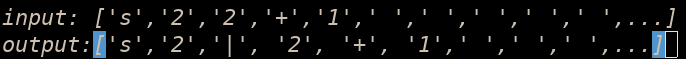
\includegraphics[scale=0.3]{png/compute1.png}
%         \item  \ \\
%         \eee{
%             \item 三进制的对齐规则(所有2位数加法):\\
%             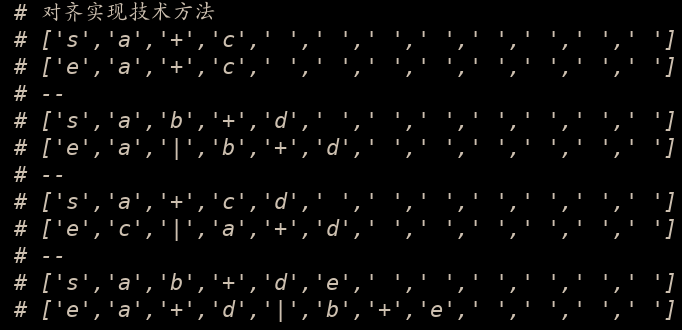
\includegraphics[scale=0.3]{png/regular-aligon.png}
%             \item 两位数加法需要对齐的情况一共就4种,分别是x位数+y位数,x,y均小于等于2,所以就有如上的规则。
%             \item 大概需要\ff{k^2}个规则数据集合
%         }
%         }
%     \end{itemize}
% \end{frame}

% \subsection{数字计算}
% \begin{frame}
%     \frametitle{数字计算:将每个分隔符分开的数字进行计算}
%     \eee{
%         \item  目标:单个数字依旧映射为本身,其中的2+1进行计算得到1 0\\
%         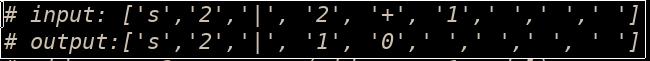
\includegraphics[scale=0.3]{png/compute.png}
%         \eee{
%             \item 三进制的计算规则(所有3位数加法规则):\\
%             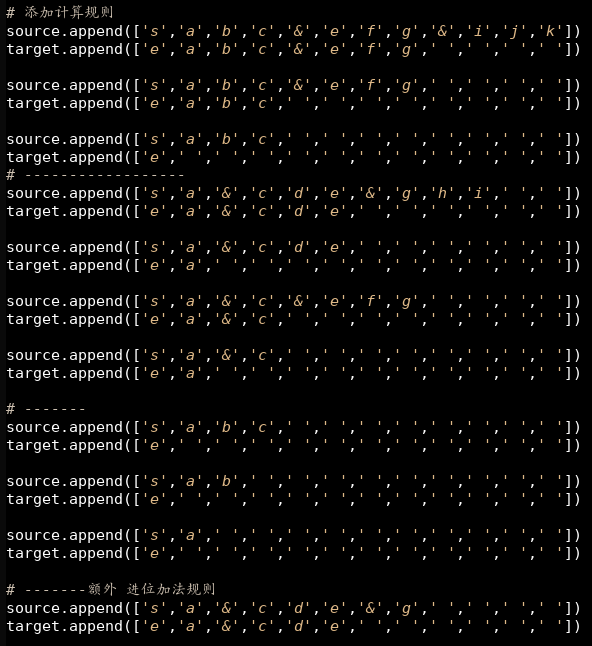
\includegraphics[scale=0.2]{png/regular_compute.png}
%         }
%     }
% \end{frame}

% \begin{frame}
%     \frametitle{数字计算:将每个分隔符分开的数字进行计算}
%     \eee{
%         \item  对规则进行迭代,每次迭代得到最后一步的计算结果\\
%         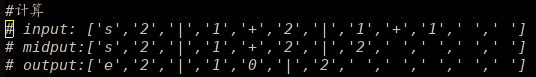
\includegraphics[scale=0.3]{png/regular_compute2.png}
%         \item 只要进行不断的规则迭代,就可以计算出每一个分隔符内的算式结果。
%         \item 对于k位的计算,需要\ff{2^k}个计算规则
%         \item 后续也可以通过拆分的思路,比如一个六位数相加可以拆成两个三位数相加,这样一来可以很大程度上减少规则,并增加效率。
%     }
% \end{frame}


% \subsection{数字进位}
% \begin{frame}
%     \frametitle{数字进位:学习进位规则,对输入数据进行进位}
%     \begin{itemize}
%         \item 目标:对计算结果进行进位\\
%         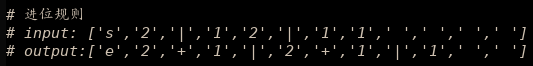
\includegraphics[scale=0.3]{png/regular_jin.png}
%         \item \ \\
%         \eee{
%             \item 三进制的进位规则(三位数加法):\\
%             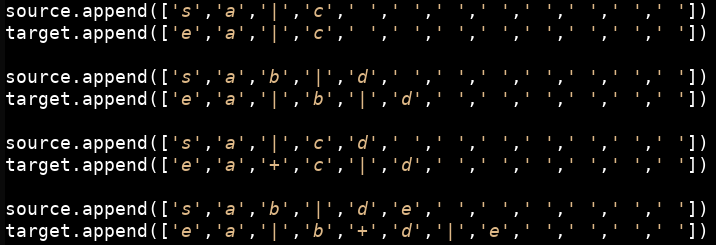
\includegraphics[scale=0.3]{png/regular-jin.png}
%             \item 进位大致需要\ff{2^k}个进位规则
%         }
%     \end{itemize}
% \end{frame}

\subsection{计划安排}
\begin{frame}
    \frametitle{具体计划}
    \begin{itemize}
        \item 论文安排
        \eee{
            \item introduction (等待修改)
            \item related work (等待修改)
            \item Methodology 
            \eee{
                \item 模型策略思路(等待修改)
                \item 模型的架构图(等待修改) 
            }
            \item experiments
            \eee{
                \item 目前实现10进制的任意五位数以内的加减运算100\%正确率(已完成)
                \item 针对别人计算不准确的问题进行比较,比如做一些减法问题(进行测试)
                \item 使用公认的数学计算数据集进行测试
                \item 对特殊问题进行分类,比如小数减大数
            }
        }
        \item 代码进度
        \eee{
            \item 大致实现各种位数的加减算法(已完成)
            \item 把稿件中提到的测试完成
            \item 做一些新例子测试
        }
        % \item 遇到的问题
        % \eee{
            % \item 一些代码上的琐碎问题。
            % \item 写论文的时候才发现需要做一些模型对比,目前还没想好如何进行比较。
        % }
    \end{itemize}
\end{frame}


% \subsection{加减法混合运算规则}

% \begin{frame}
%     \frametitle{减法在进位的时候规则比较复杂}
%     \begin{itemize}
%         \item 虽然减法规则比较复杂,但是也可以和加法类似的方法制定一套规则进行计算。
%         \item 结果展示
%     \end{itemize}
% \end{frame}

\begin{frame}
    \frametitle{模型相关信息}
    \begin{itemize}
        \item 对于一个k进制的n位加法需要的复合规则和子规则数
        \eee{
        \item 子规则数:\ff{4k^2}
        \item 进位规则数:\ff{2^{n+1}}
        \item 对齐规则数:\ff{2n^2}
        \item 运算规则数:\ff{2^n}
        } 
        合计大约:\ff{O(2^{n+1})}
        \item 模型:transformer
        \eee{
            \item 5层encode,decode
            \item 参数参数模型文件:300MB
        }
    \end{itemize}
\end{frame}

% \begin{frame}
%     \frametitle{测试}
%     \eee{
%         \item 展示测试数据的加法
%         \item 展示bug存在的原因?
%         \item 准备之后测试的代码
%     }
% \end{frame}

% \begin{frame}
%     \frametitle{下一步计划}
%     \eee{
%         \item 吧
%         % \item 进行模型相关修改
%         }
% \end{frame}

% 结束语
\section{}
\begin{frame}
	\frametitle{}
	\begin{center}
		\Huge{谢谢老师和同学们的聆听!}
	\end{center}
\end{frame}

\end{CJK*}
\end{document}
